\section{Spatial Gaussian Random Fields}
\subsection{Random Fields}
\textbf{Dette stykket om random fields må vel forbedres}

A random field is a set of random variables $\vec{Y}$ that has a distribution function 
\begin{equation} \label{eq:distribution_function}
F(Y(s_1) \leq y_1, \dots , Y(s_n) \leq y_n)
\end{equation} 

for any number $n$. A random field has typically some attribute that connects the random variables in $\vec{Y}$. Some examples of such attributes may be physical location, placement in a graph or ordering in time.

Depending on the properties of the distribution function and the setting in which it is defined, we have many different types of random fields, e.g. Markov Random Fields, Gibbs Random Fields and Conditional Random Fields, all of which may again be used with different attributes connecting the variables of the field. 

For this particular project, the main focus will revolve around a random field of type \textit{Gaussian Random Field} (GRF). A GRF is set up so that the variables $\vec{Y}$ is governed by a \textit{Gaussian process}. In addition, the Gaussian process will be assumed to be time-stationary, meaning that the Gaussian probability distributions of the process is invariant to changes in time. The variance of the process will be equal over the whole field, meaning that its spatially stationary as well. 

\subsection{Covariance functions} \label{sec:covariance_functions}

For a GRF with equal variance for all associated variables, two of them being $X$ and $Y$, we have that the covariance is defined by:
\begin{align*}
\frac{Cov( X, Y )}{\sqrt{Var( X )}\sqrt{Var( Y )}} = \frac{Cov( X, Y )}{\sigma^2} &= Corr(X, Y) \\
\implies  Cov( X, Y ) &= \sigma^2 Corr(X, Y)
\end{align*}
with $\sigma^2$ being the variance parameter of the covariance function. So the covariance of two variables are linear their pairwise correlation. \\

Evidently, by defining a covariance function to use for a Gaussian process, one achieves a expression covariance with fewer parameters to estimate or set. This simplification is desireable and acceptable for many different models, as we now are down to estimate or set what is typically a couple of parameters compared to estimating $\frac{(n-1)\cdot(n - 2)}{2}$ covariances for a Gaussian process with $n$ variables. In addition, by using a defined covariance function one is then guaranteed that the resulting covariance matrix is a \textit{positive definite matrix} \footnote{Let $M \in \mathcal{R}^n \times \mathcal{R}^n$ with $M = M^T$ be a positive definite matrix. Then, for any $\vec{z} \in \mathcal{R}^n$ we have $\vec{z}^T M \vec{z} \ > \ 0$.}. This further implies the existence of a positive definite inverse of the covariance matrix. \\

In a spatial GRF setting as we will work with, the associated variables will be linked with a spatial location. The main argument for calculating the Euclidean distance between points, denoted as $d = |s_X - s_Y|$ where $s_A$ is the spatial location for variable A. Combine this with the fact that we have the Gaussian process as time-stationary, the covariance function simplifies to a single-argument function of $d$:
\begin{equation}
Cov(X, Y) = \sigma^2Corr(X, Y) = \sigma^2C(|s_X - s_Y|) = \sigma^2C(d)
\end{equation}

Whether this simplification is reasonable comes down to model specification. However, in a spatial setting where one is modelling geophysical attributes that only change significantly in time windows of thousands of years, there is a strong argument for defining our covariance in this form. One could also look to Eidsvik et al \cite{EidsvikEtAl}, Diggle \& Lophaven \cite{DiggleEtAl} or Cressie \& Wikle \cite{CressieEtAl} for examples and justification of its use.

For the choice of covariance funcions there are many possibilities. A simple function is the exponential correlation function:
\begin{equation*}
C(d) = \text{exp}(-\frac{d}{\tau})
\end{equation*}
where $d$ is the Euclidean distance between two stochastic points X and Y in the GRF. $\tau$ is a \textit{range} parameter, describing the intensity in which a certain should affect the correlation. For easy interpretation with this function, the distance $d = 3\tau$ is of interest as the resulting correlation is exp$(-3) \approx 0.05$.
The exponential covariance function is derived as a special case of the family of \textit{Mátern covariance functions}. The Mátern covariance functions is defined in a stationary form, with distance $d$, range parameter $\tau$ and degrees of freedom $\nu$, as:
\begin{equation}
\label{eq:matern_function}
C_{\nu}(d) = \sigma^2 \frac{2^{1-\nu}}{\Gamma(\nu)}\bigg( \frac{d}{\tau} \bigg)^{\nu} K_{\nu} \bigg( \sqrt{2\nu}\frac{d}{\tau} \bigg)
\end{equation}
where $K_{\nu}$ is the modified Bessel function of the second kind. The covariance functions obtained from the Mátern family makes sample paths of an associated Gaussian process become $\nu - 1$ differentiable. The equation in (\ref{eq:matern_function}) is seemingly a complicated affair to evaluate, but it is reducable to convenient forms for many choices of $\nu$. Three of them are:
\begin{align} \label{eq:covariance_functions}
\begin{split}
\nu = \frac{1}{2}: \quad C_{\frac{1}{2}}(d) &= \sigma^2\text{exp}(-\frac{d}{\tau}) \\
\nu = \frac{3}{2}: \quad C_{\frac{3}{2}}(d) &= \sigma^2 \bigg(1  +
\frac{\sqrt{3}d}{\tau} \bigg) \text{exp}(-\frac{\sqrt{3}d}{\tau}) \\
\nu = \frac{5}{2}: \quad C_{\frac{5}{2}}(d) &= \sigma^2 \bigg(1  +
\frac{\sqrt{5}d}{\tau} + \frac{5d^2}{3\tau^2}\bigg) \text{exp}(-\frac{\sqrt{5}d}{\tau})
\end{split}
\end{align}
We recognize the exponential covariance function as the Mátern covariance function with d.o.f. $\nu = \frac{1}{2}$. This again implies that we will not have differentiable sample paths when taken from a Gaussian process using this covariance function, something that's illustrated in \textbf{eksempel/plot}.  

\begin{figure}[!htb]
\hspace{-30pt}
   \begin{minipage}{0.475\textwidth}
     \centering
     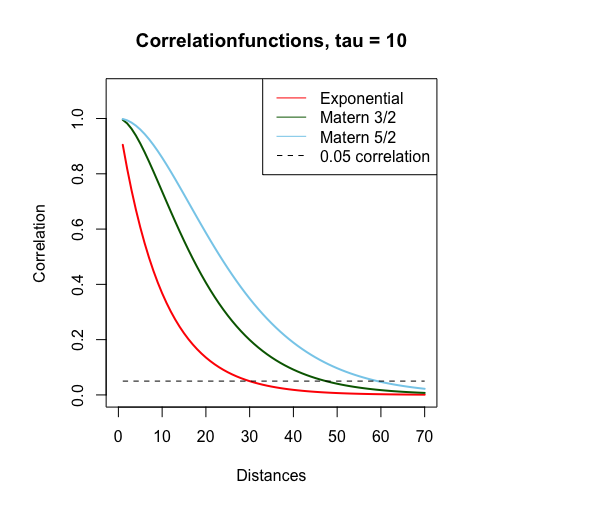
\includegraphics[width=1.3\linewidth]{figurer/correlation_tau10.png}
     \label{fig:data_original}
     \caption{Correlation with $\tau = 10$ as function of distance.}
   \end{minipage}
   \hspace{0.1pt}
   \begin{minipage}{0.475\textwidth}
     \centering
     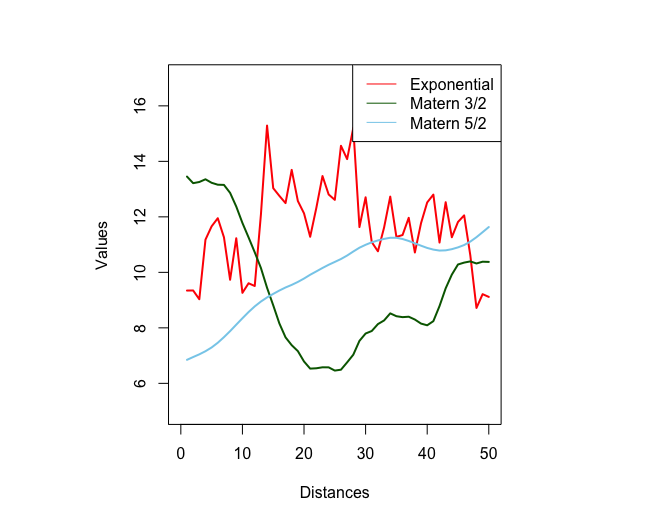
\includegraphics[width=1.3\linewidth]{figurer/sample_path-sigma10phi10.png}
	 \label{fig:data_original_reduced}
	 \caption{Sample path from model (\ref{model:hm}), $\sigma = 10$, $\phi = 10$.}
	 \end{minipage}
\end{figure}




\subsection{Gaussian processes} \label{sec:gaussian_processes}
Associated with every GRF is a underlying Gaussian process detailing the distributions of the variables contained in the field. The fundamental characterization of such a process is that all finitie-dimensional joint distributions for the variables of the process is multivariate normally distributed (MVN), and especially that each variable is normally distributed. Being distributed as a MVN, a Gaussian process is completely determined by its mean and covariance functions \textbf{ref til linstatbok}. Thus, the mean and covariance functions of a process are often a focus point in dealing with a Gaussian process. \\

Amongst the many favourable properties of MVN distributions, we also have that the best predictor for an unobserved variable in a Gaussian process is linear function of the observed variables. The predictor being a linear function of MVN distributed variables, the predictor as well is MVN distributed with an adjusted mean and covariance. \\ 

More precisely, if $\begin{bmatrix} A \\ B \end{bmatrix}$ is a vector of $n$ stochastic variables associated with a Gaussian process, meaning $\begin{bmatrix} A \\ B \end{bmatrix}$ has a distribution on the form of $\mathcal{MVN}(\begin{bmatrix} \mu_A \\ \mu_B \end{bmatrix}, \begin{bmatrix} \Sigma_{AA} & \Sigma_{AB} \\ \Sigma_{BA} & \Sigma_{BB} \end{bmatrix})$, where $\Sigma_{AB} = \Sigma_{BA}^T$ denotes the covariance between the variables in $A$ versus the variables in $B$.  given B, we have exact results for the best linear predictor. $P(A | B = b)$ will then be $MVN$, with corrected mean $\mu_{A | B}$ and variance $\Sigma_{A | B}$ as:
\begin{align}
\mu_{A | B} &= \mu_A + \Sigma_{AB}\cdot \Sigma_{BB}^{-1}\big( b - \mu_B \big) \label{eq:gaussian_conditional_expectancy} \\
\Sigma_{A | B} &= \Sigma_{AA} - \Sigma_{AB} \cdot \Sigma_{BB}^{-1} \cdot \Sigma_{BA} \label{eq:gaussian_conditional_variance}
\end{align}

In an uformal setting, one may interpret this as a linear smoothing of the parameters for the MVN distribution of $A$. Especially it's worth noting that since the covariance matrix $\Sigma_{BB}$ is positive definite, its inverse is as well, meaning that the diagonal entries of $\Sigma_{AB} \cdot \Sigma_{BB}^{-1} \cdot \Sigma_{BA}$ are all greater or equal to zero. As the variance of $P(A | B = b)$ are the diagonal elements of $\Sigma_{A|B}$, we have that the elementwise variance after conditioning on $B$ is lower or equal than with no conditioning: 
\begin{equation}
\Sigma_{A|B} = \Sigma_{AA} - \Sigma_{AB} \cdot \Sigma_{BB}^{-1} \cdot \Sigma_{BA}
\implies \Sigma_{A|B}[i, \ i]  \leq \Sigma_{AA}[i, \ i] \quad  i = 1, \dotsc, n.
\end{equation}
where $\Sigma_{AA}[i, \ i]$ denotes the entry at index $(i, i)$ in the matrix.
The equality will only hold for $\Sigma_{AB} = \mathbf{0}$, which would mean that $Cov(A, B) = 0$. Intuitively, this makes sense as then the variables of $B$ have no relation to the variables in $A$. \\

Evidently from the aforementioned property, when dealing with a Gaussian process it would be favourable to have well-defined expressions for its mean and covariance. One possible solution in the case of the process-covariance is to use a covariance function to define the covariance between variables given some criteria to evaluate.

\textbf{Model and specify the model that's been used}

\begin{figure}[!htb]
	%\hspace*{\fill}     
   \begin{minipage}{0.475\textwidth}
     \centering
     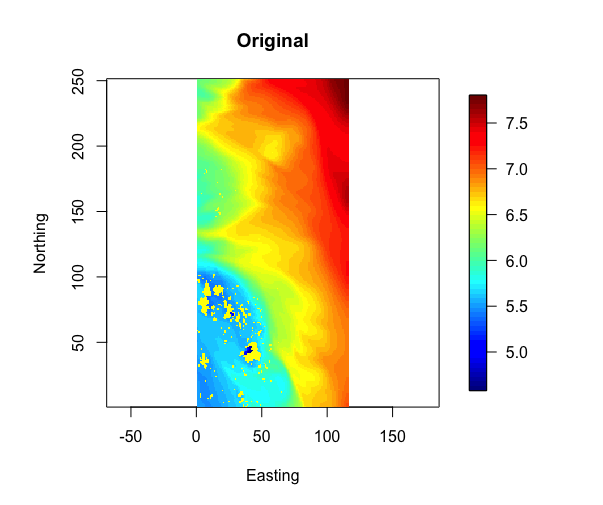
\includegraphics[width=1.25\linewidth]{figurer/original.png}
        \caption{Original termperaturedata}
        \label{fig:data_original}
   \end{minipage}
   \begin {minipage}{0.44\textwidth}
     \centering
     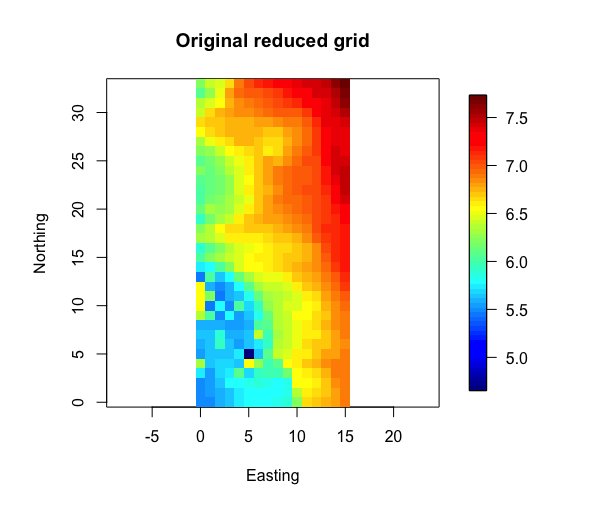
\includegraphics[width=1.3\linewidth]{figurer/original_reduced.png}
     \caption{The original data interpolated to a reduced grid for use in prediction}
	 \label{fig:data_original_reduced}
   \end{minipage}
\end{figure}

\subsection{Model design} \label{model:hm}
One common way of defining the model used to relate the process of data acquisition to the properties of the GRF is by a hierarchical model. A hierarchical model divides the spatial design model 
into three parts: 
\begin{itemize}
\item Data model - Describes the relation between process and datasampling
\item Process model - Describes the model properties of the GRF 
\item Prior model - Priors used in the case of Bayesian modelling of parameters
\end{itemize}

An example of such a model may be given for the case example used to generate the sample paths in \textbf{Ref til sample paths eksempel} \ref{fig:sample_paths}. In this model the parameters of the underlying GP is fixed, so 'Prior model' is omitted. Denoting $Z$ as the sampled data, $Y$ as the underlying GP and parameters $\mu, \tau, \sigma^2, \phi$:
\begin{itemize}
\item Data model: $Z(\vec{s}) \sim \mathcal{N}\big(F(\vec{s}) \cdot Y, \ \phi^2I(\vec{s})\big)$
\item Process model: $Y \sim \mathcal{N}\big( \vec{\mu}, \ C_Y(D, \sigma^2, \tau) \big)$ 
\end{itemize}
where $\vec{s} \in \mathcal{R}^n \times \mathcal{R}^2$ is the matrix of coordinates for the points in question, $D$ denotes a symmetric $n \times n$ matrix of distances between the points in the field, F is a matrix indicating sampling of data and $C_Y(\dots)$ the chosen covariance function. For the sample path examples in \ref{fig:sample_paths} the three covariance functions in \ref{eq:covariance_functions} have been used. \\

By using the linearity property of Gaussian variables, we may write the models as linear combinations of their means and covariances, i.e. 
\begin{itemize}
\item Data model: $Z(\vec{s}) = F(\vec{s}) \cdot Y + \epsilon, \quad \epsilon \sim \mathcal{N} \big(\vec{0},\phi^2I(\vec{s}) \big)$
\item Process model: $Y = \vec{\mu} + \rho, \quad \rho \sim \mathcal{N} \big(\vec{0}, \ C_Y(D, \sigma^2, \tau ) \big) $ 
\end{itemize}
This is a unique property of models with a GRF and Gaussian distributed errors and is of no difference compared to the first model.

\textbf{Specify the model here}

\subsubsection{GLS}
The trendfunction is another matter. As we are unaware of any data in the grid that may be related to the trend of the GRF model, the better option that is left is to estimate the trend based on the datacollection. The trendfunction is defined as a polynomial function of spatial location on the form $\mu(\vec{s}) = X(\vec{s})\vec{\beta}$, where X is a design matrix corresponding to the locations $\vec{s}$ and $\vec{\beta}$ is vector of coefficients. By doing so we may utilize results from the theory of \textit{Generalized Least Squares} (GLS) in the estimation of trend. One particular advantage of using GLM is that we are guaranteed by the Gauss-Markov Theorem that the GLR estimates is the \textit{Best Linear Unbiased Estimator} (BLUE) for the vector of coefficients $\vec{\beta}$. \\

One of two caveats with using GLR estimates is that one still need to specify the polynomial trendfunction to fit the data, meaning there's still a selection process. As the trendfunction is to specified by spatial location for this case, one must face the second caveat. The GLR estimates are the BLUE only for the data and their associated spatial location used in the estimation, giving no guarantee for the prediction of data not part of the estimates. By this, the trendfunction will be selected to be a polynomial of lower order with simple interaction between easting- and northing-coordinates. This has been chosen as an prediction far away from the sample data will typically be over- or underpredicted by an unacceptable amount using a higher-order polynomial. This is due to the covariates of said polynomial will be fitted to the data that has been sampled, which in this case will be done mainly by specified design of low regularity. In sampling designs with high regularity over the field, this is effect is handled as then the estimation will try to adapt to grid points that are within a certain distance from each other. An example of this issue is shown in figures \ref{fig:predictions_polynomials} along with the original data for comparison.  \\

When the samples are drawn from a distribution with known correlation matrix $\Omega = \sigma^2 \cdot W$, with $\sigma^2$ is constant finite variance parameter and $W$ the correlation matrix, the estimates of $\vec{\beta}$ converge in distribution to a MVN, or more precisely
\begin{equation}
\hat{\vec{\beta}} \xrightarrow[]{d} \mathcal{MVN} \big( \ \vec{\beta}, \ (X^T \Omega^{-1} X)^{-1} \big)
\end{equation}
where $X$ denotes the associated design matrix of the samples estimated.


\begin{figure}[!htb]
	%\hspace*{\fill}     
   \begin{minipage}{0.475\textwidth}
     \centering
     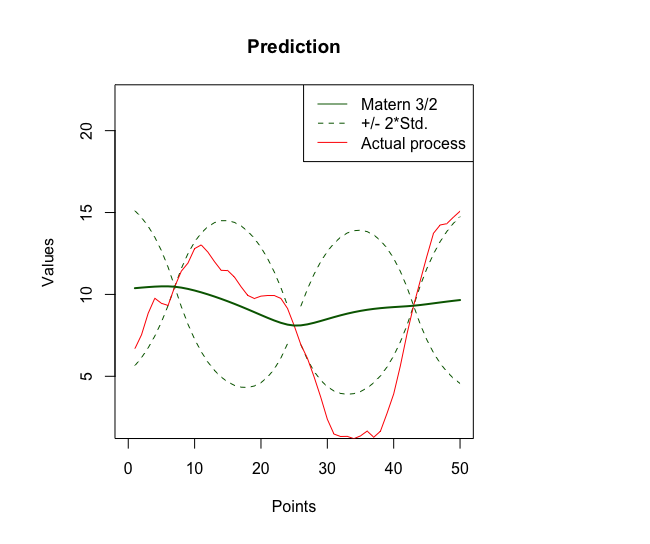
\includegraphics[width=1.25\linewidth]{figurer/prediction_325.png}
        \caption{Original termperaturedata}
        \label{fig:data_original}
   \end{minipage}
   \begin {minipage}{0.44\textwidth}
     \centering
     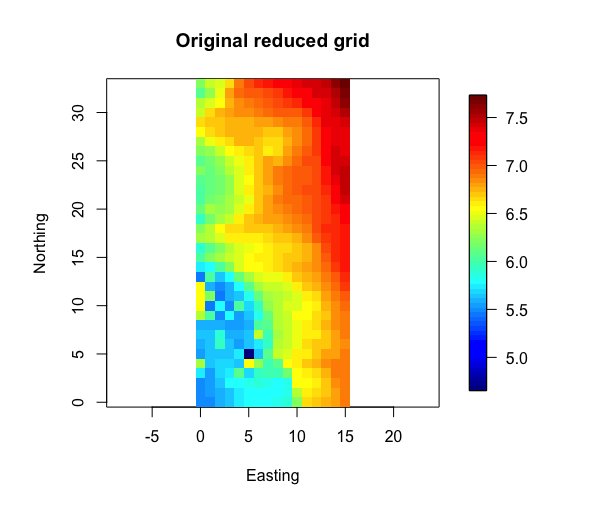
\includegraphics[width=1.3\linewidth]{figurer/original_reduced.png}
     \caption{The original data interpolated to a reduced grid for use in prediction}
	 \label{fig:data_original_reduced}
   \end{minipage}
\end{figure}

\subsubsection{Deriving the posterior GRF}
The ultimate goal of the analysis is to provide a result for the posterior distribution of the underlying Gaussian process, given some sample data, that is $P \big( Y(\vec{s}) | Z(\vec{s_0}) \big)$ where $\vec{s}$ denotes the whole coordinates of the whole field and $\vec{s_0}$ denotes the coordinates of samples obtained. This distribution is derived as 
\begin{align*}
\begin{split}
P \big( Y(\vec{s}) | Z(\vec{s_0}) \big) &= \int \int P \big( Y(\vec{s}), \sigma^2, \tau | \ Z(\vec{s_0}) \big) \ d\sigma^2 \ d\tau \\
&= \int \int P \big( Y(\vec{s}) | Z(\vec{s_0}), \sigma^2, \tau \big) \cdot P\big( \sigma^2, \tau | Z(\vec{s_0}) \big) \ d\sigma^2 \ d\tau 
\end{split}
\end{align*}
Further, we use Bayes Theorem 
\begin{align}\label{eq:posterior_prior}
\begin{split}
P\big( \sigma^2, \tau | Z(\vec{s_0}) \big) &\propto P\big( Z(\vec{s_0}) | \sigma^2, \tau \big) \cdot P\big( \sigma^2, \tau \big) \\[5pt]
&\propto P\big( Z(\vec{s_0}) | \sigma^2, \tau \big) \cdot P\big( \sigma^2 \big) \cdot P\big( \tau \big) \\[10pt]
\implies P\big( \sigma^2, \tau | Z(\vec{s_0}) \big) &= \frac{P\big( Z(\vec{s_0}) | \sigma^2, \tau \big) \cdot P\big( \sigma^2 \big) \cdot P\big( \tau \big)}{\int \int P\big( Z(\vec{s_0}) | \sigma^2, \tau \big) \cdot P\big( \sigma^2 \big) \cdot P\big( \tau \big) d\sigma^2 d\tau}
\end{split}
\end{align}
This implies that 
\begin{equation}\label{eq:grf_posterior}
\hspace*{-0.1cm}
P \big( Y(\vec{s}) | Z(\vec{s_0}) \big) = \int \int P \big( Y(\vec{s}) | Z(\vec{s_0}), \sigma^2, \tau \big) \cdot \frac{P\big( Z(\vec{s_0}) | \sigma^2, \tau \big) \cdot P\big( \sigma^2 \big) \cdot P\big( \tau \big)}{\int \int P\big( Z(\vec{s_0}) | \sigma^2, \tau \big) \cdot P\big( \sigma^2 \big) \cdot P\big( \tau \big) d\sigma^2 d\tau} \ d\sigma^2 \ d\tau
\end{equation}

An exact analytical result for the posterior found in both \ref{eq:posterior_prior} and \ref{eq:grf_posterior} may be found under the with the appropriate priors, but to acommodate any type of prior from a probability distribution, the integrals is approximated by a simple numerical procedure. This is done by discretizing the domain of $\sigma^2$ and $\tau$ and summing over the discretizied values with some weight $\Delta$ for each discretization to ensure normalization, giving an approximation as
\begin{align*}
\begin{split}
P \big( Y(\vec{s}) | Z(\vec{s_0}) \big) &\approx \frac{1}{\Pi}\sum_{\tau_i}^{n_{\tau}} \sum_{\sigma^2_j}^{n_{\sigma}} P \big( Y(\vec{s}) | Z(\vec{s_0}), \sigma^2_j, \tau_i \big) \cdot P\big( Z(\vec{s_0}) | \sigma^2_j, \tau_i \big) \cdot P\big( \sigma^2_j \big) \cdot P\big( \tau_i \big) \cdot \Delta_{ij}
\end{split}
\end{align*}
With $\Pi = \sum_{\tau_i}^{n_{\tau}} \sum_{\sigma^2_j}^{n_{\sigma}} P\big( Z(\vec{s_0}) | \sigma^2_j, \tau_i \big) \cdot P\big( \sigma^2_j \big) \cdot P\big( \tau_i \big) \cdot \Delta_{ij}$ as the normalizing constant. \\

For this integration to be performed, four distributions need to be defined: $P\big( \sigma^2_j \big)$ and $P\big( \tau_i \big)$ are priors given by the model, $P\big( Z(\vec{s_0}) | \sigma^2_j, \tau_i \big)$ is known MVN by the model specification and lastly we have that $P \big( Y(\vec{s}) | Z(\vec{s_0}), \sigma^2_j, \tau_i \big)$ is MVN by the results presented in \ref{sec:gaussian_processes} with $Y(\vec{s})$ as $A$ and $Z(\vec{s_0})$ as $B$. \\

When performing the numerical integration, it is noted that it's the mean and variance of $P\big( \sigma^2, \tau | Z(\vec{s_0}) \big)$ that's of relevance for the predictions. By similar arguments as above, one gets:
\begin{align}\label{eq:expected_variance_grf_posterior}
\begin{split}
\mathbf{E} \big( Y(\vec{s}) | Z(\vec{s_0}) \big) &= \int \int \mathbf{E} \big( Y(\vec{s}) | Z(\vec{s_0}), \sigma^2, \tau \big) \cdot \frac{P\big( Z(\vec{s_0}) | \sigma^2, \tau \big) \cdot P\big( \sigma^2 \big) \cdot P\big( \tau \big)}{\int \int P\big( Z(\vec{s_0}) | \sigma^2, \tau \big) \cdot P\big( \sigma^2 \big) \cdot P\big( \tau \big) d\sigma^2 d\tau} \ d\sigma^2 \ d\tau \\
&\approx \frac{1}{\Pi}\sum_{\tau_i}^{n_{\tau}} \sum_{\sigma^2_j}^{n_{\sigma}} \Delta_{ij} \cdot \mathbf{E} \big( Y(\vec{s}) | Z(\vec{s_0}), \sigma^2_j, \tau_i \big) \cdot P\big( Z(\vec{s_0}) | \sigma^2_j, \tau_i \big) \cdot P\big( \sigma^2_j \big) \cdot P\big( \tau_i \big) \\
\mathbf{Var} \big( Y(\vec{s}) | Z(\vec{s_0}) \big) &= \int \int \mathbf{Var} \big( Y(\vec{s}) | Z(\vec{s_0}), \sigma^2, \tau \big) \cdot \frac{P\big( Z(\vec{s_0}) | \sigma^2, \tau \big) \cdot P\big( \sigma^2 \big) \cdot P\big( \tau \big)}{\int \int P\big( Z(\vec{s_0}) | \sigma^2, \tau \big) \cdot P\big( \sigma^2 \big) \cdot P\big( \tau \big) d\sigma^2 d\tau} \ d\sigma^2 \ d\tau \\
&\approx \frac{1}{\Pi}\sum_{\tau_i}^{n_{\tau}} \sum_{\sigma_j^2}^{n_{\sigma}} \Delta_{ij} \cdot \mathbf{Var} \big( Y(\vec{s}) | Z(\vec{s_0}), \sigma^2_j, \tau_i \big) \cdot P\big( Z(\vec{s_0}) | \sigma^2_j, \tau_i \big) \cdot P\big( \sigma^2_j \big) \cdot P\big( \tau_i \big) \\\end{split}
\end{align}
with $\Pi$ defined as before. The expressions of $\mathbf{E} \big( Y(\vec{s}) | Z(\vec{s_0}), \sigma^2, \tau \big)$ and $\mathbf{Var} \big( Y(\vec{s}) | Z(\vec{s_0}), \sigma^2, \tau \big)$ is given in \ref{eq:gaussian_conditional_expectancy} and \ref{eq:gaussian_conditional_variance}.

\textbf{
Figurer
\begin{itemize}
\item cov func
\item realisasjon GRF
\item conditional grf (fix par, høy / lav korrelasjon)
\end{itemize} 
fyre inn hierarkisk modell
4.2.2-3 her
}
